\documentclass[tikz]{standalone}
\usepackage{tikz} 
\usetikzlibrary{shapes.misc,patterns,hobby}
\usepackage{pgfplots}
\usepgfplotslibrary{fillbetween}
%\usepackage[active,tightpage]{preview}  %generates a tightly fitting border around the work
%\PreviewEnvironment{tikzpicture}
%\setlength\PreviewBorder{2mm}
\usepackage{xcolor}
\definecolor{myred}{RGB}{196,19,47} 
\definecolor{myblue}{RGB}{0,139,139}

\begin{document}
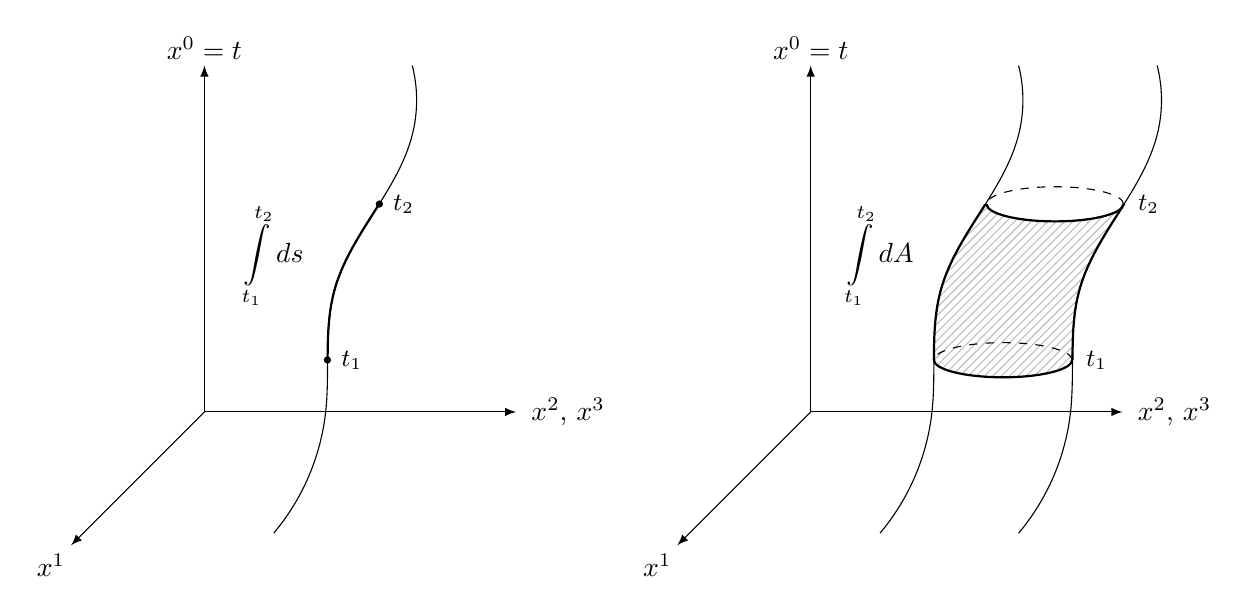
\begin{tikzpicture}[xscale=2.2,yscale=2.2,>=latex]

%Koordinatensystem (3D)
\draw[->, thin] (0,0,0) to (0,0,2);
\node at (0,0,2.3) {$x^1$};
\draw[->, thin] (0,0,0) to (1.8,0,0);
\node at (2.1,0,0) {$x^2$, $x^3$};
\draw[->, thin] (0,0,0) to (0,2,0);
\node at (0,2.1,0) {$x^0 = t$};
  

%Kurve mit fettem Abschnitt
\newcommand\kurve{(0.4,-0.7) to [curve through = { (0.7,0) (0.75,0.7) (1.2,1.6)  }] (1.2,2)}

\draw[-] \kurve;

\filldraw (0.71,0.3) circle (0.5pt); 
\node at (0.85,0.3) {\small $t_1$};
\filldraw (1.01,1.2)  circle (0.5pt); 
\node at (1.15,1.2) {\small $t_2$};

\begin{scope}[]
\clip[] (0.7,0.3) rectangle (1.02,1.2);
\draw[->, thick] \kurve;
\end{scope}

\node at (0.4,0.9) {$\displaystyle\int\limits_{t_1}^{t_2} ds$};





%Koordinatensystem (3D)
\draw[->, thin] (3.5,0,0) to (3.5,0,2);
\node at (3.5,0,2.3) {$x^1$};
\draw[->, thin] (3.5,0,0) to (5.3,0,0);
\node at (5.6,0,0) {$x^2$, $x^3$};
\draw[->, thin] (3.5,0,0) to (3.5,2,0);
\node at (3.5,2.1,0) {$x^0 = t$};
  

\newcommand\kurvee{(3.9,-0.7) to [curve through = { (4.2,0) (4.25,0.7) (4.7,1.6) }] (4.7,2)}
\newcommand\kurveee{(5.5,2) to [curve through = { (5.5,1.6) (5.05,0.7) (5,0) }] (4.7,-0.7)}
\newcommand\elipse{(4.91,1.2) ellipse (0.395 and 0.1)}
\newcommand\elipsee{(4.61,0.3) ellipse (0.399 and 0.1)}

\def\mypath{\kurvee -- \kurveee -- (3.9,-0.7)}

\path[pattern=north east lines, pattern color=gray!50] \elipsee; 
\path[draw,thick] \elipsee; 

\begin{scope}[]
\clip[] (4.2,0.3) rectangle (5.5,1.2);
\fill[color=white!] \mypath;
\fill[pattern=north east lines, pattern color=gray!50] \mypath;
\path[fill=white!] \elipse; 
\path[draw,thick] \elipse;
\path[draw,dashed,thin] \elipsee;
\draw[->, thick] \kurvee;
\draw[->, thick] \kurveee;
\end{scope}

\draw[-] \kurvee;
\draw[-] \kurveee;

\path[draw,dashed,thin] \elipse;


\node at (5.15,0.3) {\small $t_1$};
\node at (5.45,1.2) {\small $t_2$};

\node at (3.9,0.9) {$\displaystyle\int\limits_{t_1}^{t_2} dA$};


\end{tikzpicture}
\end{document}